% Chapter 3

\chapter{Herramientas utilizadas y M\'etodos} % Chapter title

\label{ch:tools} % For referencing the chapter elsewhere, use \autoref{ch:tools} 

%----------------------------------------------------------------------------------------

%\lipsum[1]

%----------------------------------------------------------------------------------------

\section{Los C\'umulos Simulados y las Muestras}
\label{sec:muestra}
El punto de partida para obtener el conjunto de c\'umulos de galaxias utilizados en este trabajo 
es una simulaci\'on cosmol\'ogica en gran escala de baja resoluci\'on. Esta simulaci\'on {\it N-body} 
cuenta con $1024^3$ part\'iculas $\sim 6.2\times10^{10}$ dentro de un box peri\'odico de $1~h^{-1}~Gpc$ de 
lado (ver Bonafede et al. 2011 por m\'as detalles). Dado su gran tama\~no, este volumen cosmol\'ogico contiene 
una muestra numerosa de 64 c\'umulos con $M_{FOF} > 1\times10^{15}  M_{\odot}$  a redshift cero ($M_{FOF}$ es 
la masa obtenida de sumar todas las part\'iculas que,
seg\'un el algoritmo {\it FOF} usado para la identificaci\'on de grupos, forman parte de un c\'umulo).  

Los 24 c\'umulos m\'as masivos (M$\sim 10^{15}$ M$_{\odot}$) en el mencionado volumen, junto a su regi\'on circundante ($5~ a~ 7~R_{vir}$), m\'as
otros cuatro menos masivos (M$\sim 10^{14}$ M$_{\odot}$) , han sido resimulados con mejor resoluci\'on, adoptando varios niveles de complejidad para 
los procesos f\'isicos involucrados: enfriamiento radiativo del gas ({\it cooling}), formaci\'on estelar, {\it feedback} de supernovas 
(estos dos por medio del modelo subgrid de Springel $\&$ Hernquist 2003) y {\it feedback} de N\'ucleos Activos ({\it AGN}). 
A estos 29 c\'umulos se los denominar\'a c\'umulos principales de la regi\'on resimulada.


Las simulaciones fueron llevadas a cabo utilizando el c\'odigo {\it TreePM-SPH GADGET-3}, una versi\'on mejorada no p\'ublica de {\it GADGET-2} 
(Springel 2005). La masa de las part\'iculas de materia oscura es de $m_{dm}=8.4\times10^8~h^{-1}M_{\odot}$, 
la masa inicial de las part\'iculas 
de gas de $m_{g}=1.6\times10^8~h^{-1}M_{\odot}$, mientras que la media de la masa inicial de las part\'iculas de estrellas 
$m_{s}$ oscila en $\sim 4.5 \times 10^7 ~h^{-1}M_{\odot}$. La longitud de suavizado o {\it softening} para las part\'iculas de estrellas, 
componente sobre la cual se basar\'a este trabajo, es  $l_{soft}=3~h^{-1}kpc$.


El modelo de {\it AGN} y su consiguiente {\it feedback}, es una versi\'on actualizada de aquel descripto en Ragone-Figueroa 
et al. 2013. En esta nueva versi\'on se ha mejorado el centrado de la part\'icula que representa al {\it BH}, lo cual ha tenido 
consecuencias directas en acercar las masas estelares de las {\it BCGs} simuladas a las mediciones observacionales. 

Sumado al conjunto de simulaciones anteriormente descriptas, se cuenta con dos c\'umulos (uno de alta y otro de baja masa) simulados
apagando el modelo de {\it feedback} de {\it AGN}.
Estos experimentos permitir\'an cuantificar la importancia del mencionado
{\it feedback} en determinar las masas finales de las {\it BCGs}.

Finalmente, los mismos dos c\'umulos mencionados en el p\'arrafo anterior fueron simulados con una mejor resoluci\'on 
para estudiar la estabilidad de los resultados. Para estos dos
casos $m_{dm}=2.5\times10^8~h^{-1}M_{\odot}$, 
$m_{g}=4.7\times10^7~h^{-1}M_{\odot}$,
$m_{s}=1.3\times10^7~h^{-1}M_{\odot}$  $l_{soft}=2~h^{-1}kpc$. 

En todas las simulaciones se asume una cosmolog\'ia de Universo plano $\Lambda$CDM, cuyo par\'ametro de 
densidad de materia es $\Omega_m=0.24$; densidad de bariones $\Omega_b=0.04$ y constante de Hubble $h=0.72$.

\medskip
A continuaci\'on se listan las distintas muestras que se utilizar\'an en este trabajo:

\begin{itemize}

\item \cmay: Muestra completa en volumen formada por los 24 c\'umulos m\'as masivos. 
\item \cmen: Muestra formada por los 5 c\'umulos principales de baja masa. 
\item \aum: Muestra Aumentada formada por {\bf CMAY}, {\bf CMEN}, m\'as
los dem\'as c\'umulos que se encuentran en las regiones resimuladas y no son principales. 
\item \agnoff: Muestra formada por los 2 c\'umulos simulados sin considerar el efecto del {\it AGN}.
\item \mr: Muestra formada por los 2 c\'umulos simulados con resoluci\'on intermedia.
\item \hr: Muestra formada por el \'unico c\'umulo simulado en alta resoluci\'on.

\end{itemize}
La Figuira ~\ref{fig:distribuciones} muestra las distribuciones de masas 
de los c\'umulos que conforman las muestras \cmay, \cmen~ y \aum

\begin{figure}[H]
 \centering
 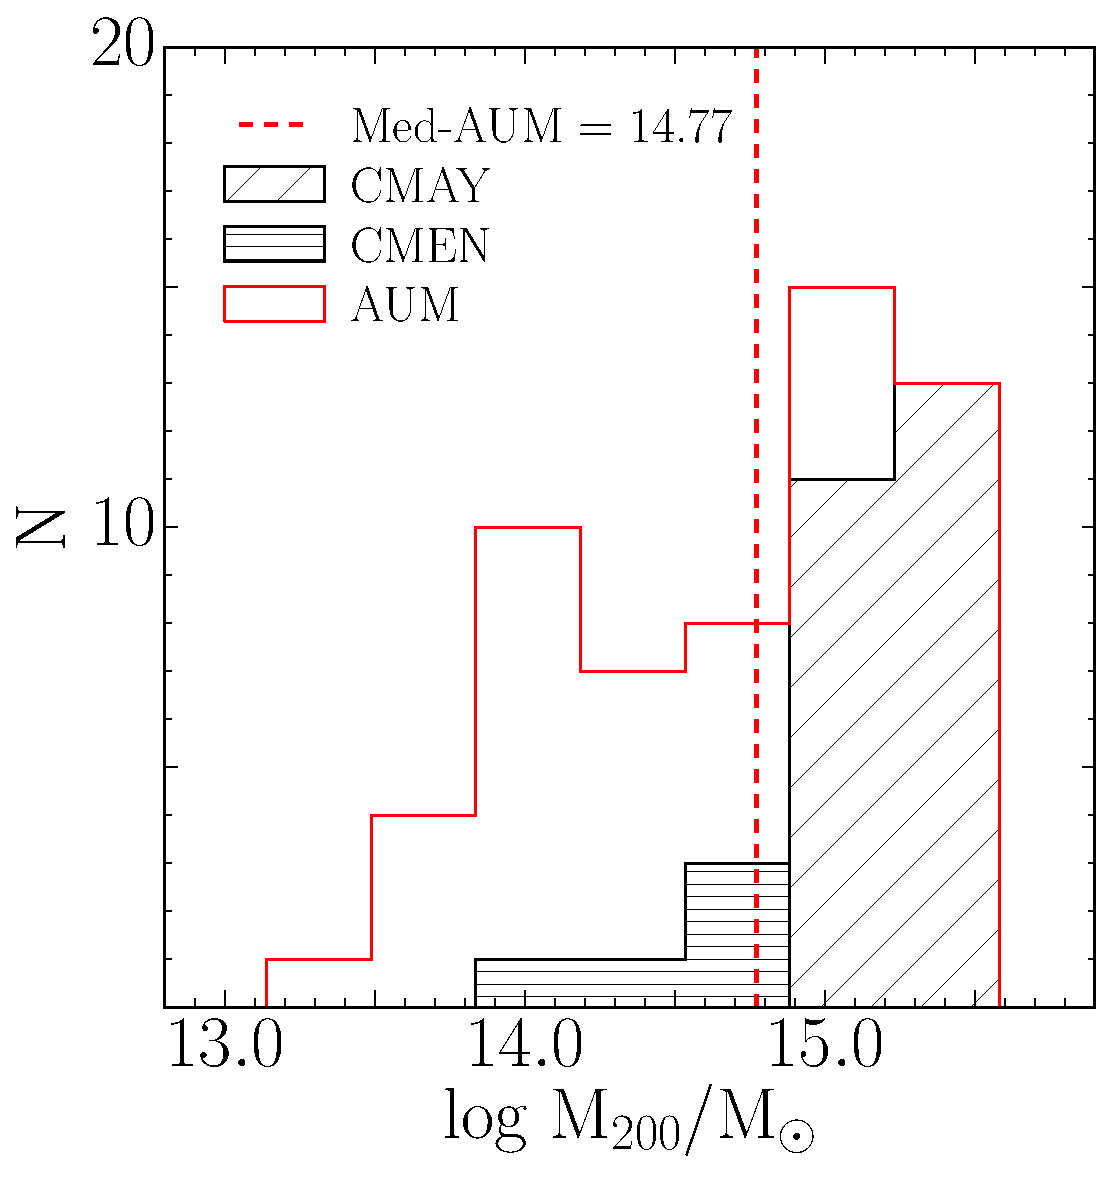
\includegraphics[height=9cm, width=9cm]{../al_final/LR/evolucion/histogramas/quilombo.pdf}
 \caption{La presete figure exhibe las distribuciones de masas M$_{200}$ de las muestras \cmay, \cmen y \aum}
 \label{fig:distribuciones}
\end{figure}


\section{Identificaci\'on de las BCGs}
El c\'odigo utilizado para realizar las simulaciones num\'ericas corre \textit{on the fly} un algoritmo {\it Friends-of-Friends} 
de identificaci\'on de halos (o c\'umulos de galaxias). Una vez identificado el c\'umulo, otro algoritmo corre sobre las part\'iculas que
forman parte del mismo para identificar sus subhalos (o galaxias sat\'elites) (Subfind, Dolag et al. 2009). Las part\'iculas de estrellas no 
ligadas a ninguna galaxia son asociadas por {\it Subfind} a la componente estelar del halo, formando as\'i un \'unico sistema BCG+Componente-Estelar-Difusa (o subhalo principal).

En este trabajo se considera que la part\'icula con m\'inimo de potencial del subhalo principal denota el centro de la BCG.
Para medir las masas de estas galaxias, tal es uno de los objetivos de este trabajo, se adoptar\'an diferentes aperturas centradas todas ellas, en el mencionado m\'inimo de potencial. 

\section{Medici\'on de la masa de las BCGs}
Observacionalmente, la obtenci\'on de las masas de las BCGs no es una medici\'on directa. El c\'alculo de la masa de las BCG se hace a
partir de una medici\'on de luminosidad y del posterior uso de un cociente masa-luminosidad.

Adem\'as de las diferentes asunciones para los cocientes masa-luminosidad utilizados, se pueden encontrar en la 
literatura diversas convenciones para medir la fotometr\'ia de las BCGs: magnitudes Petrosian, magnitudes tipo Kron, 
magnitudes obtenidas a partir de ajustes a los perfiles de brillo, magnitudes de apertura, magnitudes isofotales, 
magnitudes m\'etricas. A continuaci\'on se describen brevemente las utilizadas m\'as frecuentemente.

\begin{itemize}
\item Magnitudes Petrosian: La idea es medir una fracci\'on constante de la luz total independientemente de la distancia o posici\'on de la galaxia. Esta magnitud mide el flujo dentro del Radio Petrosian, el cual se calcula teniendo en cuenta el nivel de ruido de fondo y la forma del perfil de luz de la galaxia (Petrosian 1976; Blanton et al. 2001 y Yasuda et al. 2001). Es una medida robusta frente a variaciones de exposici\'on pero, seg\'un algunos estudios, no es apropiada para galaxias extendidas dado que subestima el flujo total. Por ejemplo seg\'un Blanton et al. 2001, la magnitud petrosian recupera casi todo el flujo para una galaxia disco pero s\'olo el $80\%$ para una galaxia con "bulge" con un perfil de de Vaucouleurs. Independientemente, Graham \& Driver (2005) encuentran que en la versi\'on utilizada por SLOAN (aperturas cirulares), la magnitud Petrosian subestima la luminosidad de galaxias con \'indices de Sersic $n=10$ en un $\sim45\%$ (0.64 mag). Bernardi et al. (2007) y Lauer et al. (2007) encuentran el mismo bias en galaxias BCGs.

\item Magnitudes Kron: Al igual que la anterior, se trata de una magnitud de "apertura escalada" en cuanto mide el flujo de la galaxia dentro de usualmente 2.5 radios de Kron. El radio de Kron se calcula teniendo en cuenta el perfil de luz (Kron 1980). No es tan robusta como la magnitud Petrosian en lo que respecta a variaciones exposici\'on-a-exposici\'on, pero es m\'as apropiada para medir el flujo total de las galaxias extendidas. Seg\'un Graham \& Driver (2005) una magnitud de Kron de una galaxia con bulge, con $n=4$, pierde $\sim 10\%$ del flujo. La dificultad para calcular esta magnitud reside en lograr una correcta medici/'on del radio de Kron, para hacerlo es necesario integrar el perfil de luz hasta radios relativamente grandes. Si la integraci\'on se corta incorrectamente el radio de Kron ser\'a mucho menor y por consiguiente se obtendr\'a un flujo equivocado, que puede llegar a ser hasta un $50\%$ menor que el real (Bernstein et al. 2002). Todos los trabajos que utilizan el software  mag\_auto de  SExtractor, calculan este tipo de magnitud (en aperturas el\'ipticas).

\item Magnitudes a partir de ajustes: En este caso hace falta ajustar alguna funci\'on al perfil de brillo de la galaxia. La magnitud de la galaxia se obtiene integrando el ajuste, en algunos casos truncando el fit en algún múltiplo del radio efectivo, en otros extrapolando a infinito. Un software muy usado en la literatura que trabaja de esta forma es GALFIT (Peng et al. 2010), el usuario puede elegir entre diferentes funciones de ajuste (Sersic, Moffat, King, Ferrer, etc.).  Bernardi+ 2013, Giallongo et al. 2014, Bellstedt+ 2016 son ejemplos de algunos trabajos en donde se usa GALFIT para obtener luminosidades de BCGs. Se pueden adem\'as encontrar trabajos en donde los autores obtienen las luminosidades de las BCGs haciendo sus propios ajustes (ej: Kravtsov et al. 2014, Gonzalez et al. 2005, Ascaso et al. 2011)

\item Magnitudes de apertura: Consiste simplemente en calcular magnitudes dentro de un radio fijo. Zhang et al. (2016) calculan por ejemplo magnitudes, y luego masas de BCGs, a partir de flujos medidos dentro de aperturas circulares de 15, 32, 50 y 60 kpc de radio.

\item Magnitudes Isofotales: Queda determinada por el flujo contenido dentro del radio donde el perfil de brillo superficial unidimensional alcanza un dado valor. Al igual que la magnitud de apertura, la magnitud isofotal posee la ventaja de ser insensible al modelo utilizado para ajustar el perfil de brillo, o a la forma del perfil de brillo. En el caso de las galaxias BCGs, esta propiedad resulta particularmente atractiva debido a la no universalidad del modelo que ajusta sus perfiles de brillo (ver \autoref{sec:perfiles}). 
Para citar algunos ejemplos, von der Linden et al. 2007 consideran que la BCG est\'a delmitada por un corte en $\mu_r=23~mag~arcsec^{-2}$ en la banda r. Fasano et al. 2010 usan el radio de la isofota $\mu_V=24~mag~arcsec^{-2}$ en la banda V. 




\end{itemize}
\section{Perfiles de brillo}
\label{sec:perfiles}
Varios trabajos pubicados recientemente han evidenciado que los perfiles de luz de algunas BCGs no pueden ser ajustados por una simple funci\'on de Sersic. 
Esto sucede cuando se verifica la presencia de una envolvente estelar extendida la cual habr\'ia sido acumulada en la parte externa de la BCG a lo largo de su formaci\'on (residuos de "mergers" o "stripping" de material de otras galaxias).

Para poder ajustar los perfiles de luz de estas galaxias extendidas hace falta sumar a la funci\'on de Sersic una componente externa, la cual puede ser otra funci\'on de Sersic o una funci\'on Exponencial (ej: Seigar et al. 2007; Donzelli et al. 2011; Ascaso et al. 2011). 

\subsection{Relaci\'on de Kormendy}
Ascaso et al. 2011 estudian una muestra de BCG a z bajo ($0.04<z<0.07$) y comparan con otra a z intermedio $0.3<z<0.6$. Encuentran que la pendiente de la relaci\'on de Kormendy crece hacia z bajos pasando de 3.3 a 4.2. Bildfell et al. 2008 tambi\'en encuentran el mismo comportamiento al comparar una muestra de BCGs a $0.15<z<0.55$  con otra local.

(Las medianas de $mu_e$ y $r_e$ en las muestras de Ascaso et al. 2011 muestran que el cambio en $mu_e$ no es significativo pero s\'i el cambio en $r_e$.)

\subsection{Par\'ametros estructurales vs. MasaBCG}
Ascaso et al. 2011 estudian  la relaci\'on existente entre las magnitudes absolutas de sus dos muestras con $n$, $r_e$ y $mu_e$. Encuentran que a una dada luminosidad las BCGs m\'as cercanas tienen $mu_e$ m\'as d\'ebil, $r_e$ m\'as grandes y par\'ametros de Sersic similares que las BCGs de la muestra a redshift intermedio.


%------------------------------------------------
%------------------------------------------------
 \section{Grasil 3D.... }

%\lipsum[6]

%----------------------------------------------------------------------------------------
